\documentclass[../main.tex]{subfiles}
\begin{document}
\chapter{Operator \& Ekspresi}

\section*{Tujuan Praktikum}
Setelah menyelesaikan praktikum ini, mahasiswa diharapkan mampu:
\begin{itemize}
  \item Memahami dan menggunakan operator aritmetika (+, -, *, /, div, mod, \%)
  \item Memahami dan menggunakan operator relasional untuk perbandingan
  \item Memahami dan menggunakan operator logika (and, or, not, \&\&, ||, !)
  \item Memahami konsep precedence dan associativity operator
  \item Menulis ekspresi kompleks dengan urutan evaluasi yang benar
  \item Menggunakan tanda kurung untuk memperjelas dan mengubah urutan evaluasi
\end{itemize}

\section{Operator Aritmetika, Relasional, Logika}
Operator aritmetika (\texttt{+}, \texttt{-}, \texttt{*}, pembagian, sisa), relasional (\texttt{\textless}, \texttt{\textless=}, \texttt{==}/\texttt{=}, \texttt{\textgreater}, \texttt{\textgreater=}), dan logika (\texttt{and}/\texttt{or}/\texttt{not} atau \texttt{\&\&}/\texttt{||}/\texttt{!}) adalah dasar evaluasi ekspresi. Perhatikan perbedaan pembagian bilangan bulat vs pecahan dan konvensi operator kesetaraan antarbahasa \parencite{pascal-tutorial-wikibooks,gnu-c-manual,cpp-reference}.

Gunakan tanda kurung untuk menegaskan maksud pada ekspresi panjang. Pecah ekspresi kompleks menjadi variabel perantara bernama agar mudah diuji. Rujuk tabel resmi operator untuk detail prioritas dan asosiasi \parencite{gnu-c-manual,cpp-op-precedence,c-op-precedence}.

\subsection{Ringkasan Operator Umum}
\begin{table}[H]
  \centering
  \caption{Operator umum lintas bahasa (ringkas)}
  \begin{tabular}{@{}llll@{}}
    \toprule
    Kategori & Pascal & C & C++ \\
    \midrule
    Aritmetika & \texttt{+ - * / div mod} & \texttt{+ - * / \%} & \texttt{+ - * / \%} \\
    Relasional & \texttt{= {\textless}{\textgreater} {\textless} {\textless}= {\textgreater} {\textgreater}=} & \texttt{== != {\textless} {\textless}= {\textgreater} {\textgreater}=} & sama dengan C \\
    Logika & \texttt{and or not} & \texttt{\&\& || !} & sama dengan C \\
    Penugasan & \texttt{:=} & \texttt{=} & \texttt{=} \\
    Inkremen & (tidak ada) & \texttt{++ --} & \texttt{++ --} \\
    \bottomrule
  \end{tabular}
\end{table}

\subsection{Operator Bitwise (C/C++)}
Operator bitwise bekerja pada representasi biner: AND (\texttt{\&}), OR (\texttt{|}), XOR (\texttt{\^{}}), NOT (\texttt{\textasciitilde}), serta pergeseran kiri/kanan (\texttt{<<}, \texttt{>>}). Ini berguna untuk masking, flags, dan operasi low-level \parencite{c-bitwise-ops,cpp-bitwise-ops}.

\begin{lstlisting}[language=C, caption={Contoh operator bitwise di C}]
#include <stdio.h>
int main(void) {
  unsigned x = 0b0101;   // 5
  unsigned y = 0b0011;   // 3
  printf("x & y = %u\n", x & y);  // 1
  printf("x | y = %u\n", x | y);  // 7
  printf("x ^ y = %u\n", x ^ y);  // 6
  printf("~x    = %u\n", (unsigned)~x);
  printf("x << 1 = %u\n", x << 1); // 10
  printf("x >> 1 = %u\n", x >> 1); // 2
}
\end{lstlisting}

\subsection{Short-Circuit dan Operator Kondisional}
Pada C/C++, operator logika \texttt{\&\&} dan \texttt{||} melakukan short-circuit — operand kanan tidak dievaluasi bila hasil sudah pasti. Operator kondisional (ternary) \texttt{?:} memilih salah satu dari dua ekspresi berdasarkan kondisi \parencite{c-conditional-operator,cpp-conditional-operator}.

\begin{lstlisting}[language=C++, caption={Short-circuit dan operator kondisional}]
#include <iostream>
using namespace std;

bool sideEffect() { cout << "called\n"; return true; }

int main() {
  bool a = false;
  if (a && sideEffect()) { /* tidak mencetak "called" */ }
  int x = a ? 1 : 2; // 2
  cout << x << "\n";
}
\end{lstlisting}

\subsection{Contoh Operator Aritmetika}
\begin{lstlisting}[language=Pascal, caption={Operator aritmetika di Pascal}]
program OperatorAritmatika;
var
  a, b: integer;
begin
  a := 10;
  b := 3;
  Writeln('Penjumlahan: ', a + b);
  Writeln('Pengurangan: ', a - b);
  Writeln('Perkalian: ', a * b);
  Writeln('Pembagian real: ', a / b:0:2);
  Writeln('Pembagian bulat: ', a div b);
  Writeln('Modulus: ', a mod b);
end.
\end{lstlisting}

\begin{lstlisting}[language=C, caption={Operator aritmetika di C}]
#include <stdio.h>
int main(void) {
  int a = 10, b = 3;
  printf("Penjumlahan: %d\n", a + b);
  printf("Pengurangan: %d\n", a - b);
  printf("Perkalian: %d\n", a * b);
  printf("Pembagian real: %.2f\n", (float)a / b);
  printf("Pembagian bulat: %d\n", a / b);
  printf("Modulus: %d\n", a % b);
  return 0;
}
\end{lstlisting}

\begin{lstlisting}[language=C++, caption={Operator aritmetika di C++}]
#include <iostream>
using namespace std;

int main() {
  int a = 10, b = 3;
  cout << "Penjumlahan: " << a + b << "\n";
  cout << "Pengurangan: " << a - b << "\n";
  cout << "Perkalian: " << a * b << "\n";
  cout << "Pembagian real: " << (float)a / b << "\n";
  cout << "Pembagian bulat: " << a / b << "\n";
  cout << "Modulus: " << a % b << "\n";
}
\end{lstlisting}

\subsection{Contoh Operator Relasional dan Logika}
\begin{lstlisting}[language=Pascal, caption={Operator relasional dan logika di Pascal}]
program OperatorRelasionalLogika;
var
  a, b: integer;
  hasil: boolean;
begin
  a := 10;
  b := 5;
  { Operator Relasional }
  hasil := a > b;
  Writeln('a > b: ', hasil);
  hasil := a = b;
  Writeln('a = b: ', hasil);
  hasil := a <> b;
  Writeln('a <> b: ', hasil);
  { Operator Logika }
  hasil := (a > b) and (b > 0);
  Writeln('(a > b) and (b > 0): ', hasil);
  hasil := (a < b) or (b > 0);
  Writeln('(a < b) or (b > 0): ', hasil);
  hasil := not (a = b);
  Writeln('not (a = b): ', hasil);
end.
\end{lstlisting}

\begin{lstlisting}[language=C, caption={Operator relasional dan logika di C}]
#include <stdio.h>
int main(void) {
  int a = 10, b = 5;
  int hasil;
  // Operator Relasional
  hasil = a > b;
  printf("a > b: %d\n", hasil);
  hasil = a == b;
  printf("a == b: %d\n", hasil);
  hasil = a != b;
  printf("a != b: %d\n", hasil);
  // Operator Logika
  hasil = (a > b) && (b > 0);
  printf("(a > b) && (b > 0): %d\n", hasil);
  hasil = (a < b) || (b > 0);
  printf("(a < b) || (b > 0): %d\n", hasil);
  hasil = !(a == b);
  printf("!(a == b): %d\n", hasil);
  return 0;
}
\end{lstlisting}

\begin{lstlisting}[language=C++, caption={Operator relasional dan logika di C++}]
#include <iostream>
using namespace std;

int main() {
  int a = 10, b = 5;
  bool hasil;
  // Operator Relasional
  hasil = a > b;
  cout << "a > b: " << hasil << "\n";
  hasil = a == b;
  cout << "a == b: " << hasil << "\n";
  hasil = a != b;
  cout << "a != b: " << hasil << "\n";
  // Operator Logika
  hasil = (a > b) && (b > 0);
  cout << "(a > b) && (b > 0): " << hasil << "\n";
  hasil = (a < b) || (b > 0);
  cout << "(a < b) || (b > 0): " << hasil << "\n";
  hasil = !(a == b);
  cout << "!(a == b): " << hasil << "\n";
}
\end{lstlisting}

\section{Precedence vs Order of Evaluation}
Precedence dan asosiasi menentukan bagaimana ekspresi dikelompokkan tanpa tanda kurung. Order of evaluation (urutan evaluasi operand) adalah konsep terpisah; di C/C++ beberapa operator tidak menentukan urutan evaluasi sehingga efek samping ganda dapat memicu perilaku tak terdefinisi. Gunakan tanda kurung dan variabel perantara untuk kejelasan \parencite{gnu-c-manual,cpp-op-precedence,c-op-precedence,c-order-of-eval,cpp-order-of-eval}.

\subsection{Penjelasan Precedence dan Associativity}
Precedence (prioritas) menentukan operator mana yang dievaluasi terlebih dahulu dalam ekspresi tanpa tanda kurung. Operator dengan precedence lebih tinggi dievaluasi sebelum operator dengan precedence lebih rendah. Associativity (asosiativitas) menentukan arah evaluasi ketika operator memiliki precedence yang sama: kiri-ke-kanan atau kanan-ke-kiri.

Untuk memastikan urutan evaluasi yang benar dalam ekspresi kompleks, gunakan tanda kurung eksplisit. Ini meningkatkan keterbacaan dan menghindari kesalahan logika yang sulit dilacak.

\subsection{Tabel Precedence Operator}
\begin{table}[H]
  \centering
  \caption{Precedence operator (tinggi ke rendah)}
  \begin{tabular}{@{}llll@{}}
    \toprule
    Level & Operator & Associativity & Kategori \\
    \midrule
    1 & \texttt{()}, \texttt{[]} & kiri-ke-kanan & Pengelompokan, array \\
    2 & \texttt{++}, \texttt{--} (postfix) & kiri-ke-kanan & Increment/decrement \\
    3 & \texttt{!}, \texttt{not}, unary \texttt{+}, \texttt{-} & kanan-ke-kiri & Unary \\
    4 & \texttt{*}, \texttt{/}, \texttt{\%}, \texttt{mod}, \texttt{div} & kiri-ke-kanan & Multiplikatif \\
    5 & \texttt{+}, \texttt{-} & kiri-ke-kanan & Additif \\
    6 & \texttt{<}, \texttt{<=}, \texttt{>}, \texttt{>=} & kiri-ke-kanan & Relasional \\
    7 & \texttt{==}, \texttt{!=}, \texttt{=}, \texttt{<>} & kiri-ke-kanan & Kesetaraan \\
    8 & \texttt{\&\&}, \texttt{and} & kiri-ke-kanan & Logika AND \\
    9 & \texttt{||}, \texttt{or} & kiri-ke-kanan & Logika OR \\
    10 & \texttt{=}, \texttt{:=}, \texttt{+=}, \texttt{-=} & kanan-ke-kiri & Penugasan \\
    \bottomrule
  \end{tabular}
  \\Sumber: \parencite{gnu-c-manual,cpp-op-precedence,c-op-precedence}
\end{table}

\subsection{Sketsa Pohon Ekspresi}
Untuk memvisualisasikan bagaimana precedence bekerja, perhatikan pohon ekspresi berikut yang menunjukkan urutan evaluasi operator dari bawah (prioritas tinggi) ke atas (prioritas rendah):

\begin{figure}[H]
  \centering
  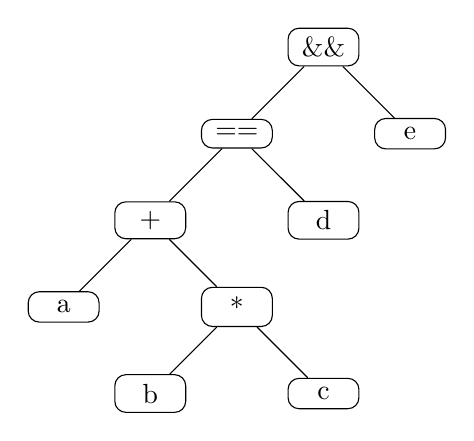
\begin{tikzpicture}[level distance=1.1cm, sibling distance=2.2cm]
    \tikzstyle{n}=[draw, rounded corners, minimum width=9mm, align=center]
    \node[n]{\&\&}
      child{ node[n]{==}
        child{ node[n]{+}
          child{ node[n]{a} }
          child{ node[n]{*}
            child{ node[n]{b} }
            child{ node[n]{c} }
          }
        }
        child{ node[n]{d} }
      }
      child{ node[n]{e} };
  \end{tikzpicture}
  \caption{Precedence: \texttt{*} \textgreater{} \texttt{+} \textgreater{} \texttt{==} \textgreater{} \texttt{\&\&}}
\end{figure}

Pada pohon di atas, operator \texttt{*} (perkalian) berada paling bawah sehingga dievaluasi terlebih dahulu, diikuti \texttt{+}, lalu \texttt{==}, dan terakhir \texttt{\&\&}. Ini menunjukkan ekspresi: \texttt{(a + b * c) == d \&\& e}.

\subsection{Contoh Demonstrasi Precedence}
\begin{lstlisting}[language=Pascal, caption={Precedence operator di Pascal}]
program PrecedenceDemo;
var
  a, b, c, hasil: integer;
begin
  a := 10;
  b := 5;
  c := 2;
  { Perkalian (*) memiliki precedence lebih tinggi dari penjumlahan (+) }
  hasil := a + b * c;
  Writeln('a + b * c = ', hasil);        { Output: 20 }
  Writeln('(a + b) * c = ', (a + b) * c); { Output: 30 }
  
  { Operator dengan precedence sama: evaluasi kiri-ke-kanan }
  hasil := a - b + c;
  Writeln('a - b + c = ', hasil);        { Output: 7 }
  Writeln('a - (b + c) = ', a - (b + c)); { Output: 3 }
end.
\end{lstlisting}

\begin{lstlisting}[language=C, caption={Precedence operator di C}]
#include <stdio.h>
int main(void) {
  int a = 10, b = 5, c = 2;
  int hasil;
  // Perkalian (*) memiliki precedence lebih tinggi dari penjumlahan (+)
  hasil = a + b * c;
  printf("a + b * c = %d\n", hasil);        // Output: 20
  printf("(a + b) * c = %d\n", (a + b) * c); // Output: 30
  
  // Operator dengan precedence sama: evaluasi kiri-ke-kanan
  hasil = a - b + c;
  printf("a - b + c = %d\n", hasil);        // Output: 7
  printf("a - (b + c) = %d\n", a - (b + c)); // Output: 3
  
  // Operator relasional dan logika
  hasil = a > b && b > c;
  printf("(a > b) && (b > c) = %d\n", hasil); // Output: 1 (true)
  return 0;
}
\end{lstlisting}

\begin{lstlisting}[language=C++, caption={Precedence operator di C++}]
#include <iostream>
using namespace std;

int main() {
  int a = 10, b = 5, c = 2;
  int hasil;
  // Perkalian (*) memiliki precedence lebih tinggi dari penjumlahan (+)
  hasil = a + b * c;
  cout << "a + b * c = " << hasil << "\n";        // Output: 20
  cout << "(a + b) * c = " << (a + b) * c << "\n"; // Output: 30
  
  // Operator dengan precedence sama: evaluasi kiri-ke-kanan
  hasil = a - b + c;
  cout << "a - b + c = " << hasil << "\n";        // Output: 7
  cout << "a - (b + c) = " << a - (b + c) << "\n"; // Output: 3
  
  // Operator relasional dan logika
  bool cek = (a > b) && (b > c);
  cout << "(a > b) && (b > c) = " << cek << "\n"; // Output: 1 (true)
}
\end{lstlisting}

Contoh di atas menunjukkan bagaimana precedence memengaruhi hasil evaluasi. Tanpa tanda kurung, \texttt{a + b * c} dievaluasi sebagai \texttt{a + (b * c)} karena perkalian memiliki prioritas lebih tinggi. Dengan tanda kurung eksplisit \texttt{(a + b) * c}, urutan evaluasi berubah dan menghasilkan nilai berbeda.

\section{Perilaku Tak Terdefinisi: Contoh Klasik}
Hindari ekspresi dengan efek samping berulang pada objek yang sama tanpa pemisahan yang jelas.

\begin{lstlisting}[language=C, caption={Contoh UB: increment dan penggunaan berulang}]
#include <stdio.h>
int main(void) {
  int i = 1;
  int a = i++ + i++; // tak terdefinisi di C: jangan lakukan ini
  printf("%d\n", a);
}
\end{lstlisting}

Pisahkan langkahnya agar portabel dan jelas:
\begin{lstlisting}[language=C]
int i = 1;
int a = i;
int b = i + 1;
i += 2;
int sum = a + b; // aman dan jelas
\end{lstlisting}

\section{Troubleshooting Umum}
\begin{itemize}
  \item \textbf{Hasil tak konsisten}: cek efek samping ganda dan urutan evaluasi.
  \item \textbf{Pembagian bulat vs real}: pastikan tipe operand sesuai (cast eksplisit bila perlu).
  \item \textbf{Kesetaraan}: Pascal \texttt{=} vs C/C++ \texttt{==}.
  \item \textbf{Bitwise vs logika}: bedakan \texttt{\&} dengan \texttt{\&\&}, \texttt{|} dengan \texttt{||}.
\end{itemize}

\section{Rangkuman Materi}
\begin{itemize}
  \item Operator aritmetika, relasional, logika, dan bitwise lintas bahasa.
  \item Short-circuit (\texttt{\&\&}, \texttt{||}) dan operator kondisional (ternary).
  \item Perbedaan \emph{precedence/associativity} vs \emph{order of evaluation} serta konsekuensi efek samping.
  \item Contoh perilaku tak terdefinisi (UB) dan pola aman dengan variabel perantara.
  \item Tabel precedence ringkas dan pohon ekspresi untuk memvisualisasi pengelompokan.
\end{itemize}

\end{document}
